% Chunked-LUT TLG decomposition (Fig. for Section III-B).
% Build: cd paper/figures/src && pdflatex fig_tlg_decomp.tex && \
%   mv fig_tlg_decomp.pdf ../
\documentclass[border=2pt]{standalone}
\usepackage{mathptmx}
\usepackage{tikz}
\usetikzlibrary{arrows.meta,positioning,calc,decorations.pathreplacing,fit}

\definecolor{navy}{HTML}{1F3A5F}
\definecolor{tlgred}{HTML}{A83232}
\definecolor{redfill}{HTML}{F4DADA}

\begin{document}
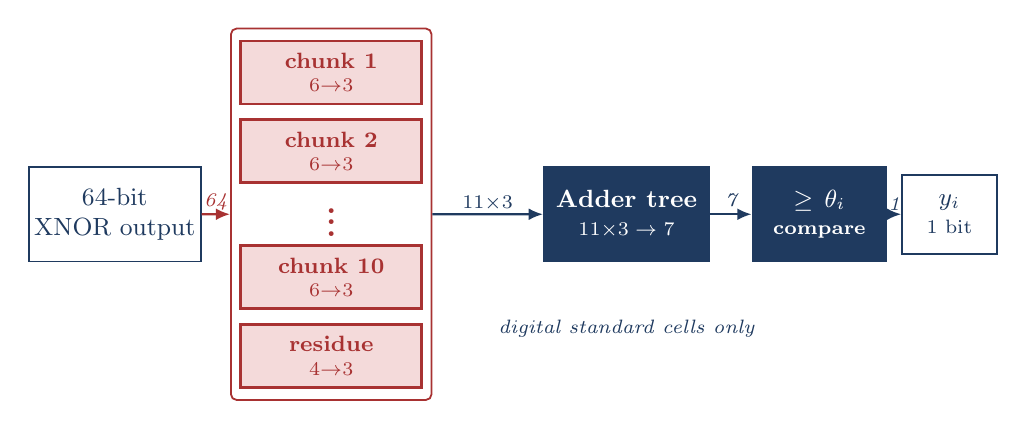
\begin{tikzpicture}[
    font=\rmfamily,
    >={Latex[length=1.8mm,width=1.5mm]},
    line width=0.65pt,
    source/.style={draw=navy, fill=white, text=navy, line width=0.7pt,
                   minimum width=19mm, minimum height=12mm, align=center,
                   inner sep=2pt, font=\rmfamily\small},
    tlg/.style={draw=tlgred, fill=redfill, text=tlgred, line width=1.0pt,
                minimum width=23mm, minimum height=8mm, align=center,
                inner sep=2pt, font=\rmfamily\footnotesize\bfseries},
    logic/.style={draw=navy, fill=navy, text=white, line width=0.7pt,
                  minimum width=21mm, minimum height=12mm, align=center,
                  inner sep=2pt, font=\rmfamily\small\bfseries},
    outbox/.style={draw=navy, fill=white, text=navy, line width=0.7pt,
                minimum width=12mm, minimum height=10mm, align=center,
                inner sep=2pt, font=\rmfamily\small},
    sig/.style={draw=navy, line width=0.75pt, ->},
    redsig/.style={draw=tlgred, line width=0.85pt, ->},
    lbl/.style={font=\rmfamily\scriptsize\itshape, text=navy, inner sep=1pt},
    redlbl/.style={font=\rmfamily\scriptsize\itshape, text=tlgred, inner sep=1pt},
    note/.style={font=\rmfamily\scriptsize\itshape, text=navy, align=center,
                 inner sep=1pt},
  ]

  % Input and chunked-LUT stage.
  \node[source] (xnor) at (-3.20,-0.25) {64-bit\\XNOR output};

  \node[tlg] (c1)  at (-0.45, 1.55) {chunk 1\\[-1pt]\scriptsize $6{\to}3$};
  \node[tlg] (c2)  at (-0.45, 0.55) {chunk 2\\[-1pt]\scriptsize $6{\to}3$};
  \node[text=tlgred, font=\rmfamily\large\bfseries] (dots) at (-0.45,-0.25) {$\vdots$};
  \node[tlg] (c10) at (-0.45,-1.05) {chunk 10\\[-1pt]\scriptsize $6{\to}3$};
  \node[tlg] (c11) at (-0.45,-2.05) {residue\\[-1pt]\scriptsize $4{\to}3$};

  \node[draw=tlgred, rounded corners=2pt, inner xsep=3pt, inner ysep=4pt,
        fit=(c1)(c2)(dots)(c10)(c11)] (chunkbox) {};
  \draw[redsig] (xnor.east) -- (chunkbox.west)
    node[redlbl, midway, above] {64};

  % Conventional digital accumulation and compare.
  \node[logic] (adder) at (3.30,-0.25) {Adder tree\\[-1pt]\scriptsize $11{\times}3 \to 7$};
  \node[logic, minimum width=17mm] (cmp) at (5.75,-0.25) {$\geq\,\theta_i$\\[-1pt]\scriptsize compare};
  \node[outbox] (yout) at (7.40,-0.25) {$y_i$\\[-1pt]\scriptsize 1 bit};

  \draw[sig] (chunkbox.east) -- (adder.west)
    node[lbl, midway, above] {$11{\times}3$};
  \draw[sig] (adder.east) -- (cmp.west)
    node[lbl, midway, above] {7};
  \draw[sig] (cmp.east) -- (yout.west)
    node[lbl, midway, above] {1};

  \node[note, anchor=north, align=center]
    at ($(adder.south)+(0,-0.68)$)
    {digital standard cells only};
\end{tikzpicture}
\end{document}
